\documentclass{article}
\usepackage[utf8,latin1]{inputenc}
\usepackage{cite}
\usepackage{amsmath,amssymb,amsfonts}
\usepackage{algorithmic}
\usepackage{graphicx}
\usepackage{textcomp}
\usepackage{xcolor}
\usepackage{cite}
\usepackage{tikz}
\usepackage{subcaption}
\usepackage{tabularx}
\usepackage{url}
\usepackage{nicefrac}
\usetikzlibrary{positioning}
\usetikzlibrary{shapes,arrows}
\usepackage[switch,modulo,pagewise]{lineno}
%\linenumbers

\title{Deep Learning Framework for structural analysis of  single particle cryo-EM maps}


\date{February 2019}

\newcommand{\xf}{\mathbf{x}}
\newcommand{\yf}{\mathbf{y}}
\newcommand{\zf}{\mathbf{z}}
\newcommand{\pf}{\mathbf{p}}

\begin{document}
\Large
\begin{center}Tel Aviv University \\
The Raymond and Beverly Sakler Faculity of Exact Sciences\\
School of Computer Science\\
\textbf{\large  Deep Learning Framework for structural analysis of  single particle cryo-EM maps} \\
(Ph.D. Reserarch Proposal) \\
Rozanov Mark \\
Supervisor: Haim J. Wolfson \\
\end{center}
\normalsize

\section{Abstract}
Cellular processes are performed and regulated by assemblies of macromolecules. 
Full understanding of the function, associations and dynamics of  such
assemblies comes from their detailed atomic structural description. 
Traditionally structural analysis of a complex is made by integration of the results of various experimental techniques: X-ray crystallography, NMR, cryo electron microscopy (cryo-EM)  and others.
The output of a cryo-EM experiment is a 3D density map.
In recent years,  vast progress was achieved in obtaining high-resolution (3.5\AA~ and below) cryo-EM maps.
However,  modelling an atomic structure from a cryo EM  map remains difficult.
For high-resolution maps  researchers mostly rely on
methods developed for X-ray crystallography. 
Modelling protein assemblies into medium resolution maps is usually based on image processing techniques and has still not yet achieved good performance.

Parallel to the advances in Cryo-EM in the last decade, deep neural networks achieved remarkable performance in various 2D and 3D image processing tasks. 
Those include Convolutional Neural Networks (CNNs) for image classification, Fully Convolutional Networks (FCN) for semantic image segmentation, Variational AutoEncoders (VAEs) and Generative Adversarial Networks (GANs) for realistic image generation.

We propose a Deep Learning Analysis Framework (DLAF) for integrative structural analysis of cryo-EM maps.
The proposed framework integrates 3D imaging information from a cryo-EM map with existing sequence and structural data.
Deep Convolutional Networks  are used to locate structural motifs within a map.
CNNs are trained on a dataset adjusted to a specific problem.
This adjustment is  done using the sequence and structural data.
Realistic cryo-EM map simulation plays a key role in the presented approach.
While the simulation of experimental maps is crucial for DLAF, it is also a valuable tool for development and analysis of algorithms which work with cryo-EM and can contribute a lot to the structural bioinformatics community.
Preliminary results of our study show that CNN are capable to successfully detect amino acids in high-resolution cryo-EM maps.
We also developed a realistic simulation of an experimental cryo-EM map using an adversarial deep learning approach.
\section{Introduction}
\subsection{General}
Cellular processes are performed and regulated by assemblies of macromolecules. Such assemblies, which are often referred to as molecular machines \cite{Alberts1998TheMachines}, vary widely in their lifespan, size, activity and dynamics. Complete understanding of the function and dynamics of an assembly is derived from its detailed atomic structure.
Structural characterization of macromolecular assemblies  represents a major challenge in structural biology.
While there exist contemporary experimental techniques, each suffers from  drawbacks. X-ray crystallography (\cite{Drenth1999PrinciplesSeparation}) is limited by the ability to grow suitable crystals and to build molecular models into large unit cells; NMR spectroscopy (\cite{Riek2002SolutionStructures}) is restricted by size; electron microscopy (\cite{BAUMEISTER2000624}), affinity purification (\cite{Bauer2003AffinityComplexes}), yeast two hybrid (\cite{PARRISH2006387}) and FRET spectroscopy (Truong and Ikura 2001) suffer from low resolution of the corresponding structural information.
Single particle cryo electron microscopy (s.p. cryo EM) plays an important role in biomolecular structure determination.
For many years data obtained by s.p. cryo-EM was of low resolution due to technical limitations. However, recent technical improvements such as direct electron detectors combined with modern computational methods for data acquisition and image processing, coined as "resolution revolution" have led  to an ability to obtain s.p. cryo-EM images of high resolution, i.e., 4 {\AA} and better, \cite{Venien-Bryan2017}, \cite{Dubochet2018}. 
While the gold rush of high resolution s.p. cryo-EM data continues, the task of determining an atomic structure from s.p. cryo-EM image remains very labourous and can be thought of like a master artwork.
 Next, we provide a more detailed description of  few computational methods that can be used in atomic structure determination from a s.p. cryo-EM image.

\subsection{Protein Structure Modelling from cryo-EM maps}
\paragraph{Intermediate resolution }
Most of the effort in modeling protein structures into intermediate resolution ($5 - 10`$ {\AA}) maps focuses on locating structural motives.
PowerFit \cite{C.P.vanZundert2015} and Multifit \cite{Tjioe2011} compute candidate  locations  for predefined structural fragments within a map.
EMatch  \cite{Dror2006}, SSEHunter \cite{Baker2007a}, StrandRoller \cite{Si}, and EMBuilder \cite{Zhou2017} use geometry calculations and a template-based search
to identify secondary structures.
Machine Learning algorithms are widely used to identify secondary structure, e.g.  SSELearner \cite{Si2012} (SVM) and \cite{Li2016} (Deep CNNs).
EMatch \cite{Dror2006} and MULTIFIT \cite{Tjioe2011} exploit   structural motives detection in order to model the  entire protein complex.
The modelling is based on rigid fitting of template protein structures into a cryo-EM map, while detected structural fragments serve as anchors.

At resolutions better than $4-5$ {{{\AA}}} de novo modeling techniques are being exploited. 
In addition to  adaptations of the standard X-ray crystallography modeling methods, which tend to be time consuming, several de-novo modeling techniques have been developed to deal specifically with cryoEM density maps\cite{DiMaio2016}.  Pathwalking \cite{Chen2016} detects first pseudo-atom anchors and then applies the travelling salesperson (TSP) combinatorial optimization algorithm to detect the protein backbone.
MAINMAST \cite{Terashi2018} detects a set of anchor points and calculates the backbone by applying  a minimun spanning tree (MST) approach.
A recently published method \cite{Zhou2017a}  fits short sequence based structure fragment templates into the density map and applies a Monte Carlo simulated annealing procedure to detect a set of mutually compatible fragments.  
\subsection{Deep Learning}
Deep neural networks are powerful learning models that achieve excellent performance in visual and
speech recognition problems [9, 8].
Neural networks achieve high performance because they can
express an arbitrary computation that consists of a modest number of massively parallel nonlinear steps.
\paragraph{Convolutional neural networks} (CNNs) were proposed by Yann LeCun in 1989 for zip code recognition \cite{Y.LeCunB.BoserJ.S.DenkerD.HendersonR.E.Howard1989}.
A CNN consists of alternating convolutional and pooling layers optionally followed by fully connected layers.
The first and last layers are  the input and  output layer respectively, while the other layers are referred to as hidden layers.

Formally, a CNN of depth $D$  is a composition of $D$  parametrized functions $\{f_1,\cdots,f_D\}$, which maps an input vector $\xf$ to an output vector $\yf$:
\begin{equation}\label{cnn1}
	\yf = f(\xf) = f_D(\zf,w_D,b_D) \circ, \ldots, \circ f_1(\xf,w_1,b_1),
\end{equation}
where $w_k$ and $b_k$ are the weights and biases vectors for the function $f_k$.  The functions $f_k$ are the previously mentioned layers.

Given a set of labeled data pairs $\{(\xf^i,\yf^i)\}_{i=1}^M$, the training process of a CNN defined by \eqref{cnn1} is a process of a numerical solution of the optimization problem:
\begin{equation}
\begin{array}{l}
\mbox{Find } \{w_k, b_k\}_{k=1}^D \mbox{ which minimize:} \\
\frac{1}{M} \sum\limits_{i=1}^{M}d\left(f(\xf_i),\yf_i\right),
\end{array}
\end{equation}
where $d(\cdot,\cdot)$ is the loss function expressing a penalty for an incorrect classification.
For a comprehensive discussion of CNNs the reader is referred to  \cite{Goodfellow2016}.
\newline
\newline
The development of the techniques below was motivated by the observation that the current amount of experimental cryo-EM data is not sufficient for DL training and thus the data has to be augmented by data from other sources.
\paragraph{Domain shift.}
If a CNN is used on data with  features distribution different from the data it was trained on, its performance degrades.
The problem is known as \textbf{domain shift}. 
In this case a \textbf{domain adaptation} technique is required.
In \textbf{transfer learning }  \cite{Oquab } a pretrained net is fine tuned by training on a relatively small dataset, which has feature distribution resembling the query data.
The main principle of \textbf{adversarial domain adaptation} techniques (\cite{Tzeng2017}, \cite{Ganin2017}) is to train a CNN such that in a prediction phase of the network only the features  which are common to the train and the test domains are used.

\subsection{Proposed Research}
We propose to develop and apply deep learning algorithms for locating structural motifs in cryo EM maps of high and medium resolution.
While all algorithms utilize deep CNN for 3D object detection and classification, the detection goal depends on the  cryo EM map resolution:
\begin{enumerate}%[(i)]
    \item CNN for detection of Amino Acids in  High Resolution ($2-4$ {\AA}) maps.
    \item CNN for annotation of SSEs (helices, beta-strands)  in  Medium Resolution ($4-6$ {\AA}) maps.
     \item CNN for detection of functionaly significant regions,  such as Binding Sites  in  Medium Resolution  ($4-6$ {\AA}) maps.
\end{enumerate}
We  anticipate a  lack of comprehensive experimental training data set for all three CNNs mentioned above, we intend to address it as follows:
\begin{enumerate}%[(i)]
    \item For  High Resolution ($2-4$ {\AA}) maps CNN is trained on existing crystallography data. 
    Since the X-ray crystallography  technique differs from single particle cryo-EM a domain shift problem is anticipated.
    We suggest to handle it  using Deep Domain Confusion \cite{Tzeng2014} technique. 
    \item We shell develop a realistic cryo-EM simulations using the VAE-GAN net (\cite{Larsen2016} , \cite{Wu}).
\end{enumerate}

In the final stage we shall attempt to develop a novel algorithm for de-novo modelling of protein structures from cryo-EM maps at appropriate resolution.



\section{Research Goals And Significance }

\subsection{Detection of anchor amino acids in high resolution cryo-EM density maps }
We propose a Deep Learning based method for the detection of 
high confidence anchor amino acid residues in high resolution cryo-EM maps.
We focus on detection of  {\bf amino acid anchors} in the density map, namely having knowledge of even a relatively small number of amino acids, whose identity and location has been established with high confidence.
Reliable prior detection of amino acid anchors can be used to guide the various de-novo modeling methods, as well as serve as a starting point for the development of novel methods.
In particular, it could lead to the development of novel techniques, which do not require prior segmentation of the EM density map.
The lack of sufficient experimental data required for  the training stage is the main expected pitfall. 
We propose two different approaches to cope with the shortage of experimental data.

 
\paragraph{Integrating X-ray crystallography data with cryo-EM for structure determination}.

X-ray crystallography is an invaluable tool for revealing the  three-dimensional structure of molecules. 
Contemporary online databases: CSD ( \url{http://www.ccdc.cam.ac.uk}) ,PDB (\url{http:// www.rcsb.org/pdb}, and  PDBe (\url{http://www.ebi.ac.uk/pdbe/node/1}) contain more than 100,000 biological macromolecules.


While having the same form of a 3D matrix of density values, Xray crystallography data differs from cryo EM data in the conditional distribution of the outputs given the inputs.
The problem is known as \textit{dataset shift}, \cite{Quinonero-Candela2010 }.
This is due to different principles of cryo-EM and X-ray crystallography experiments, from specimen preparation to data processing, (see Figure ~\ref{f:em_cryst} and \cite{Zanotti2016}, \cite{Zeng2018},\cite{Wang2017},\cite{Venien-Bryan2017} for details).

The proposed algorithm is to train a CNN on large amount of X-ray data ( \textit{source domain}) with the existing cryo-EM data (\textit{target domain}) .
A \textbf{domain adaptation} procedure will be applied to compensate for  the difference  between the source and the target domains. 


The presented  algorithm contains a novel approach  to  cryo-EM and X-ray processing in which both data types complement each other in the task of atomic structure determination.
Running the algorithm on new experimental data will reveal structural properties at high precision, which is crucial for revealing the functionality and for drug design.



\begin{figure}[!ht]

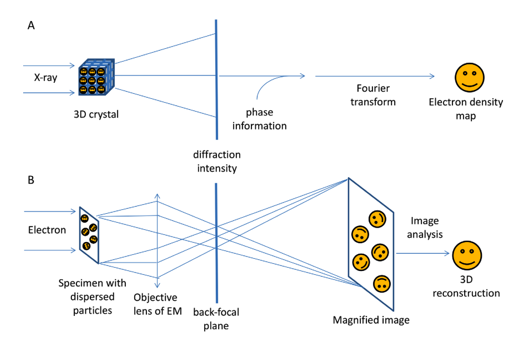
\includegraphics[width=0.95\textwidth]{pics/em_cryst}
\caption{Technical difference between X-ray crystallography and single particle cryo-EM. }\label{f:em_cryst}
\end{figure}

\begin{figure}[!ht]

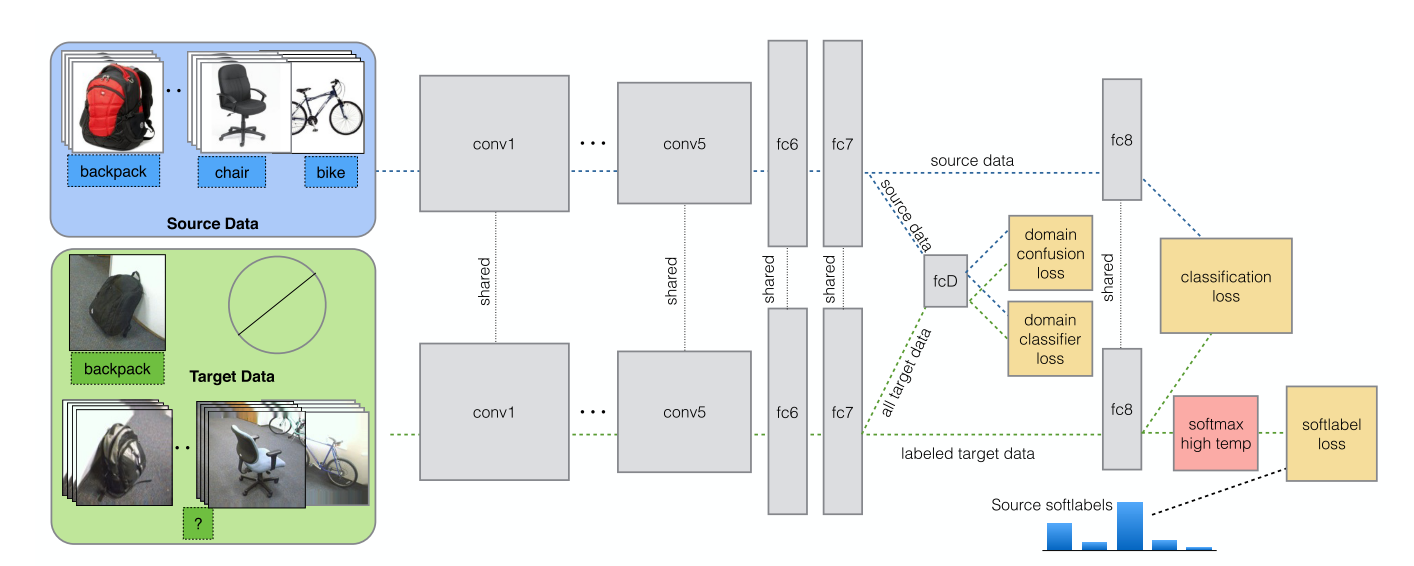
\includegraphics[width=0.95\textwidth]{pics/dom_conf_1}
\caption{Deep Domain Confusion Architecture }\label{f:dom_conf_1}
\end{figure}



\subsection{Simulating cryo-EM maps using Generative Adversarial Network}
Our previous work on the AAnchor algorithm \cite{Rozanov2018AAnchor:Maps}, showed that augmenting a training dataset by  synthetic data improves a classification CNN performance. 
Contemporary models for generating   synthetic cryo EM maps from atomic structure are incapable to generate realistic data.
We propose to use Generative Adversarial Networks  with Variation AutoEncoder (VAE-GAN) to create cryo-EM maps which are indistinguishable from experimental ones.
GANs  and VAEs are proven deep learning techinques for generating 2D and 3D images.
Reliable cryo EM map simulation is of great significance for the protein structural modelling task. 
In addition to augmenting the training dataset as in our case, such simulation is capable of improving performance of template matching based modelling methods: PowerFit \cite{C.P.vanZundert2015}, MultiFit \cite{Tjioe2011}, EMatch \cite{Dror2006}, and others. 



\subsection{Annotating Secondary Structure in Medium Resolution ($4 -6$ {{\AA} } ) cryo-EM maps}

We propose a Deep Learning based method for the detection  of Secondary Structure Elements (SSE) in medium resolution cryo-EM map.
Locating SSEs (helices, beta-strands) is of high importance to protein modelling and number of methods have been developed for the task.
One group of the developed  methods uses image  processing tools, for locating cylinder-like (helices) and plane (beta-sheets) structures, \cite{Baker2007a},  \cite{Jiang2001}, \cite{Rusu2012}, \cite{Yu2008}.
Another family of SSE detections methods uses ML approach \cite{Ma2012RENNSH:Maps} \cite{Si2012a} including  deep CNNs \cite{Velankar2012}, \cite{Li2016},\cite{Ma2003}, \cite{Mostosi2019AutomatedNetworks}.


While the above mentioned methods relied solely on structural features, we propose an \textbf{integrative} method  which 
incorporates protein sequence information as well.
The query protein sequences are used to search for homologs with known structure.
A realistic cryo-EM simulation will be used to create a dataset from these homologous structures.
The new dataset should have a similar features distribution as the query map.
The created synthetic dataset will be used for fine tunnig of the detection CNN.

\subsection{ Detection of binding sites (BSs)  in medium resolution ($4 -6 ${{\AA} } ) cryo-EM density maps}
Whilst de-novo protein modeling from a median resolution map remains an unresolved problem, we focus on locating BSs.  
Our task is to mark voxels in the cryoEM map which belong to a protein-protein interface or  a protein binding site.
Since  BSs dictate the molecular function, they are usually more evolutionary conserved and tolerate less flexibility than less functionally important parts of a protein structure. 
A deep learning approach will benefit from both of the above mentioned  properties.
Evolutionary conservation leads to a greater amount of similar structures in existing databases. 
Due to the limited flexibility, structures under search should be similar or nearly similar to those in a database. 
Locating  BSs is an important step towards full atomic structure determination, since it provides information about protein tertiary structure and separation to domains.
From a biological point of view  BSs are key to understanding protein functionality
\paragraph{Integrative algorithm for finding conserved structures in cryo-EM maps.}
The existing vast amount of data about conserved structures, is hard to utilize, since it  belongs to different domains.
Resolved protein structures are represented as lists of atom positions.
Results of cryo-EM experiments are given in a form of a 3D matrix of electron density.
Sequence data is represented as a list of chains, where each chain is an ordered sequence from an alphabet of twenty letters.  
To address the challenge of utilizing all three types of data, we suggest a deep learning algorithm architecture which combines a standard Convolutional Neural Network with Generative Adversarial Network, Transfer Learning and Multiple Sequence Alignment.

\begin{minipage}{0.209\textwidth}
{\Large Existing Simulation - pdb2mrc}
        \begin{tikzfigure}
           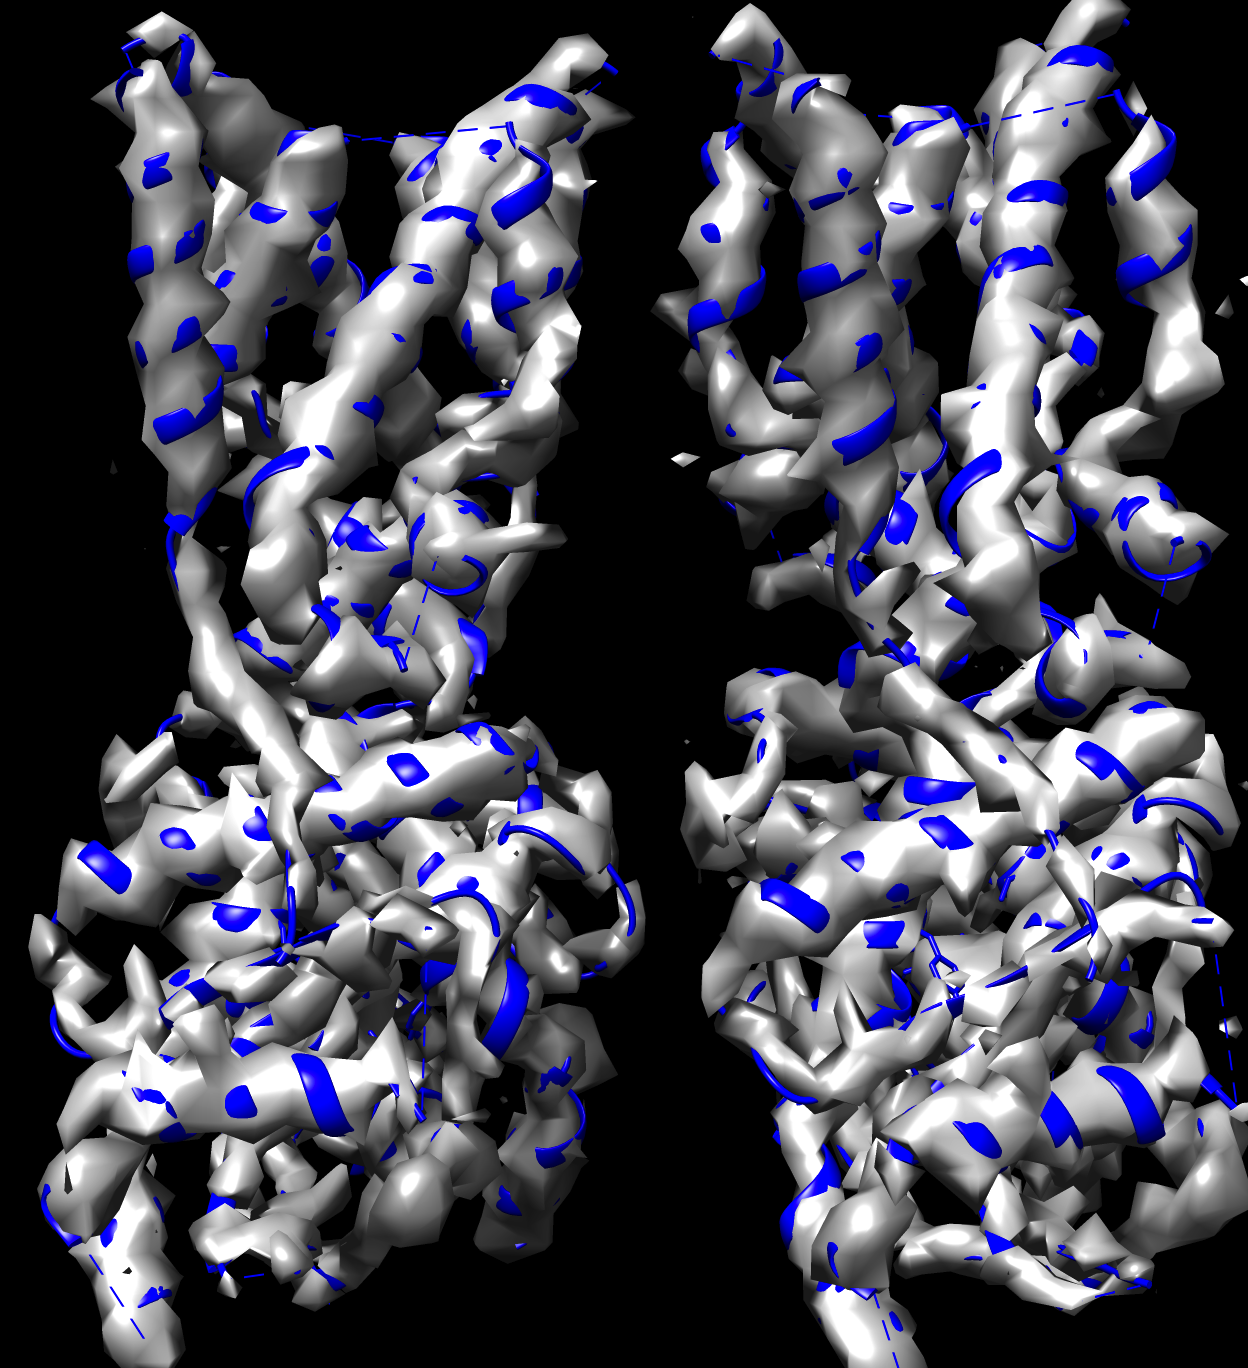
\includegraphics[width=0.9\textwidth]{mol_map.png}
        \end{tikzfigure}
\end{minipage}
\begin{minipage}{0.209\textwidth}
{\Large Real Map - EMD0505}
        \begin{tikzfigure}
           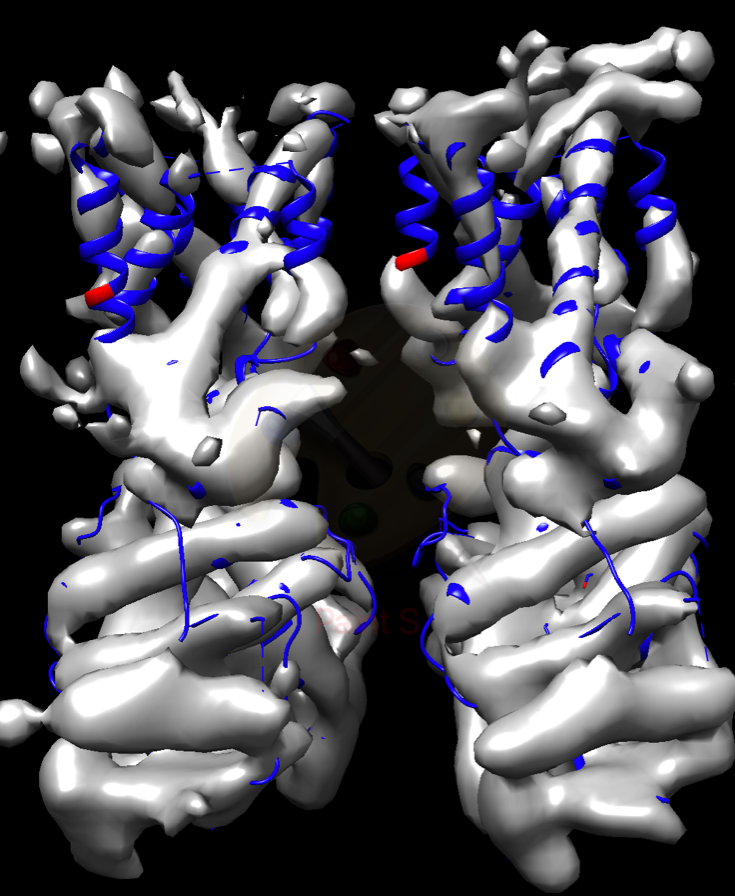
\includegraphics[width=0.9\textwidth]{real_map.png}
        \end{tikzfigure}
\end{minipage}
\begin{minipage}{0.209\textwidth}
{\Large Deep Simulation -cryoGAN}
        \begin{tikzfigure}
           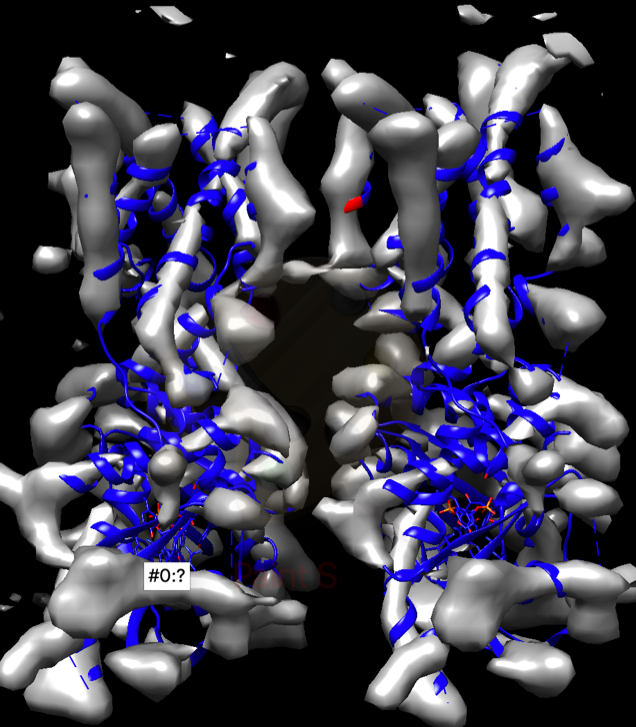
\includegraphics[width=0.9\textwidth]{gen_map.png}
        \end{tikzfigure}
\end{minipage}
\section{Future Research }
Our main goal is to develop a tool for extracting structural information from a cryoEM map at various resolutions.
Specifically, given a cryoEM map of an assembly, we intend to localize regions in the map of known and important atomic structure.
Such regions are called anchors.
The structure of the anchors will depend on the map resolution.
For very high-resolution maps (3 Angstroms and better) amino acids and aromatic rings will be identified. 
For intermediate  resolution maps (4- 6 Angstroms and better)  binding sites and protein-protein interfaces will be identified.

The general strategy will be to train a classification Convolution Neural Network (CNN) for each anchor type. Given a small cube of cryoEM  density a  classification CNN  will assign a label to the cube. 
Cubes where an atomic structure was identified with high confidence will be labelled as anchors.  The whole map will be searched for anchors by transforming a classification CNN into a Full Convolutional Network (FCN).
\subsection{Detecting Amino Acids in very high resolution maps.}\label{s:aa_task}
We should continue to develop the techique of Amino Acid detection in High Resolution Maps.
Given an electron density map of a protein/macromolecular assembly, our task is to detect voxels in this map, which correspond to the location of the centres of mass of specific amino acids.
The goal is to report only those amino acids, which have been detected with high confidence, nicknamed "anchors".
The detection procedure consists of  extracting small cubes from a map and applying  a \textit{selective classifier}  to each cube.
\paragraph{Selective Classification}. A selective classification is a classification with a reject option. A \textit{selective classifier} is a pair of functions $f(x)$, called the \textit{classifier}, and $g(x)$ is  called \textit{selection  function}. The classification of a proposal $x$ is as follows:
\begin{equation}
(f,g)(x) = \left\{ \begin{array}{lcl}
f(x) & if & g(x) = 1 \\
NONE & if & g(x) = 0 \\
\end{array}
\right.
\end{equation}

We anticipate that integrating sythetic and X-ray crystallography data will result in  improvement of  the performance of our algorithm.

\subsubsection{Training Phase}
In a training process the parameters of a selective classification are adjusted by running backpropagation algorithm on a large amount of labeled data. 
The main limitation of the training phase is small amount of high resolution cryo EM maps.
There are two additional data sources which we try to use in the training phase:
\begin{enumerate}
    \item Crystallographic data. PDBe database \cite{Velankar2012} contains tens of thousands of electron density maps.
    \item Synthetic Data i.e., cryo-EM maps obtained by simulation program from a given atomic structure.  
\end{enumerate}
Both sources mentioned above suffer from the \textbf{domain shift}, i.e., the difference in the data distribution between train and test sets. 
To address this issue, two \textbf{domain adaptation} approaches are proposed to bridge the gap between the source and target domains: utilizing crystallography data (Section ~\ref{s:fut_xray}) and semi-supervised approach (Section ~\ref{s:fut_semi_super}) .


\subsubsection{Utilizing X-ray Crystallography Data }\label{s:fut_xray}
We suggest to use the Domain Confusion architecture presented in \cite{Hoffman2017}, see Fig. \ref{f:dom_conf_1}.
Up to  date for most of the molecular   complexes in cryo-EM dataset  X-ray data can be found for the same molecule or its close homolog.
Meaning that a one-to-one correspondence is available for entries in the target and source domain.
We will adjust the domain confusion network to take an advantage of the above fact by adding a new loss function member.

\subsection{Semi-Supervised Deep Learning Approach for Anchors Detection }\label{s:fut_semi_super} 
Semi-Supervised Deep Learning Approach presented at Fig ~\ref{f:semi_super} utilizes realistic cryo-EM map simulation for Anchors detection.
The query protein sequence is used to detect atomic models of structural homologs. 
This can be done by employing local alignment search tools (BLAST, PSI-PLAST, HHPred) or retrieving known structures from the protein family according to existing hierarchical classifications (SCOP \cite{Hubbard1999}, CATH \cite{Orengo1997}).
Retrieved homolog structures are fed to  the VAE-GAN simulation to create realistic cryo-EM maps (see Section  ~\ref{s:fut_gan} for details).
Created synthetic cryo-EM maps together with atomic models are used for fine tuning of the pretrained neural network. 
Anchors locations are obtained by running a fine-tuned network on the query map.
The presented approach has a number of advantages:
\begin{itemize}
    \item Sequence information is utilized in the anchor location task.
    \item Using homolog structures ensures that the training dataset and the query map have similar feature distributions.
    \item Training datasets of arbitrary size can be created.
\end{itemize}

\subsection{Annotating Secondary Structure in a Medium Resolution ($4 -6${\AA} ) cryo-EM maps}
The task is to assign each voxel in the qiven cryo-EM map to one of the three secondary structures: helix, beta-strand, coil.
This task is known as \textbf{semantic segmentation}.
The voxel is classified according to the cube in  the 3D map which surounds it.
Classification CNN converted to   Fully Convolutional Network  (FCN) is used.
The classification CNN is pretrained on a set of experimental cryo-EM maps  of medium resolution.
Fine tunnig achieved by training the last two layers on simulated data set as shown on Fig.~\ref{f:semi_super} and Section~\ref{s:fut_semi_super}




\begin{figure}
  \centering
	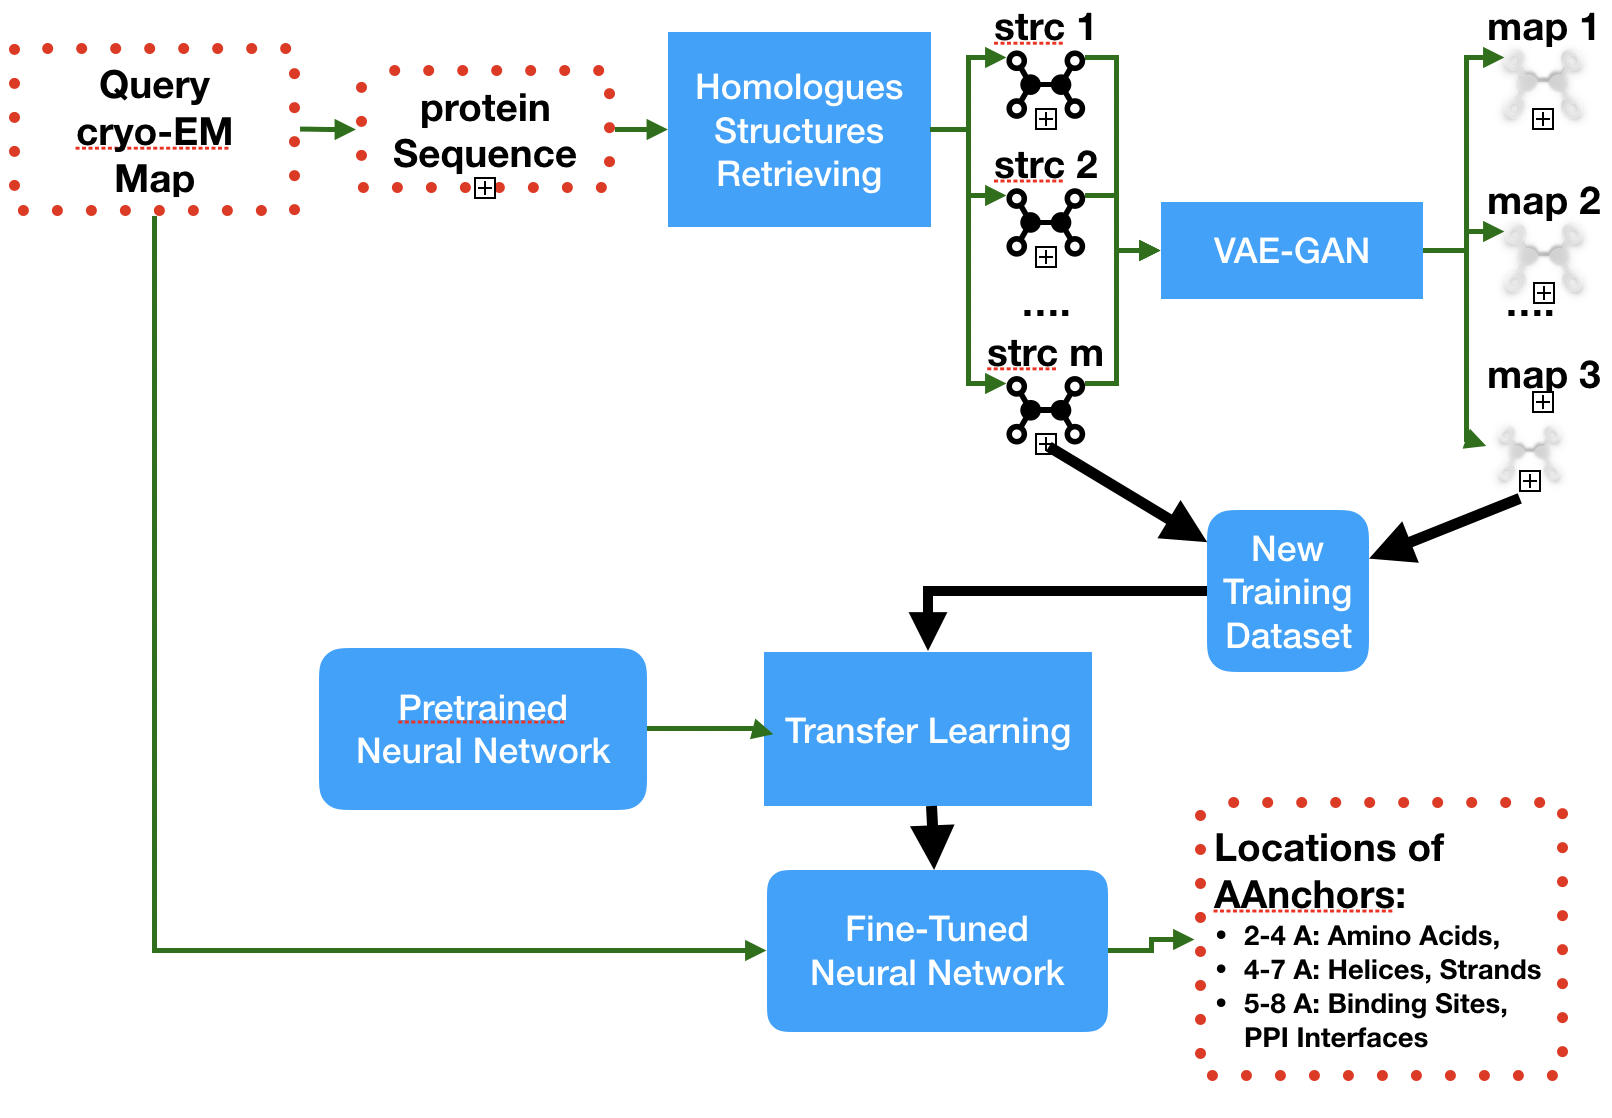
\includegraphics[scale=0.4]{picsnew/semi_super.png}
  \caption{Semi Supervised ML Algorithm for Locating Anchors}\label{f:semi_super}
\end{figure}



\subsection{Locating  Binding Sites in medium resolution cryo-EM maps }\label{bs_task}
Proteins with similar function often have active sites which are structurally similar. 
Active site structures  are usually conserved during evolution.
Despite the above facts, locating an active site for an unknown functionality is a challenging task.
This is due to the wide structual diversity of protein active sites.
Their  structural diversity can be reduced by existing sequence analysis algorithms. 
We propose a  four -phased algorithm for integrative location of binding sites - Fig.\ref{f:det_scheme4}.

In the \textbf{sequence analysis} phase possible reqions of binding sites are located in the query protein sequence.
This  can be done using traditional tools for finding conserved regions (conSurf \cite{Ashkenazy2010}  and others  \cite{Capra2007},  \cite{Fischer2008},  \cite{Rausell2010},  \cite{Lopez2011} ) or new Deep Learning Tools  (DeepBind \cite{Alipanahi2015}, and others \cite{Cui2019},  \cite{Chen2011ATPsiteResidues}).
Atomic models are created from the located sequence regions using existing modelling tools (Modeller , Rosetta).
In the \textbf{simulation} phase generated atomic models
are fed to VAE-GAN to create realistic synthetic cryo-EM maps of  expected binding  sites.
In the \textbf{transfer learning phase}  a pretrained CNN is fited to the new dataset, which consists of generated atomic models and synthetic cryo-EM maps.
Finally, in the \textbf{search} phase, the query map is fed to the fine-tuned neural network. 

\subsection{Calibration}
 In the anchor detection tasks( amino acids detection  Section \ref{s:aa_task} and binding site detection Section \ref{bs_task}) the confidence of reported detections matters.
 The goal is to filter out picks with confidence below a predefined threshold (say $80 \%$).
 This can be done by \textbf{calibration} of a detection network, using post-training methods such as \textbf{temperature scaling} \cite{Guo2017}.
 Another approach is to estimate the uncertainty of the neural network prediction by its training history \cite{Geifman2018}.
 
\subsection{Realistic cryo EM  Simulation : Generative Adversarial Network}\label{s:fut_gan}
Realistic cryo EM map simulation is the core of the algorithm presented above.
In the preliminary work we have developed cryo-GAN (Section \ref{s:c-GAN}).
The simulation uses Variational AutoEncoder (VAE) architecture combined with Generative Adversarial Network (GAN) to create  a cryo-EM map of an atomic structure.
While the preliminary results show that cryo-GAN is able to generate realistic cryo-EM maps, additional performance evaluation is required.
Moreover, we plan futher develop the simulation to make it a useful tool for algorithm developers working with cryo electron microscopy.


\begin{figure}
  \centering
	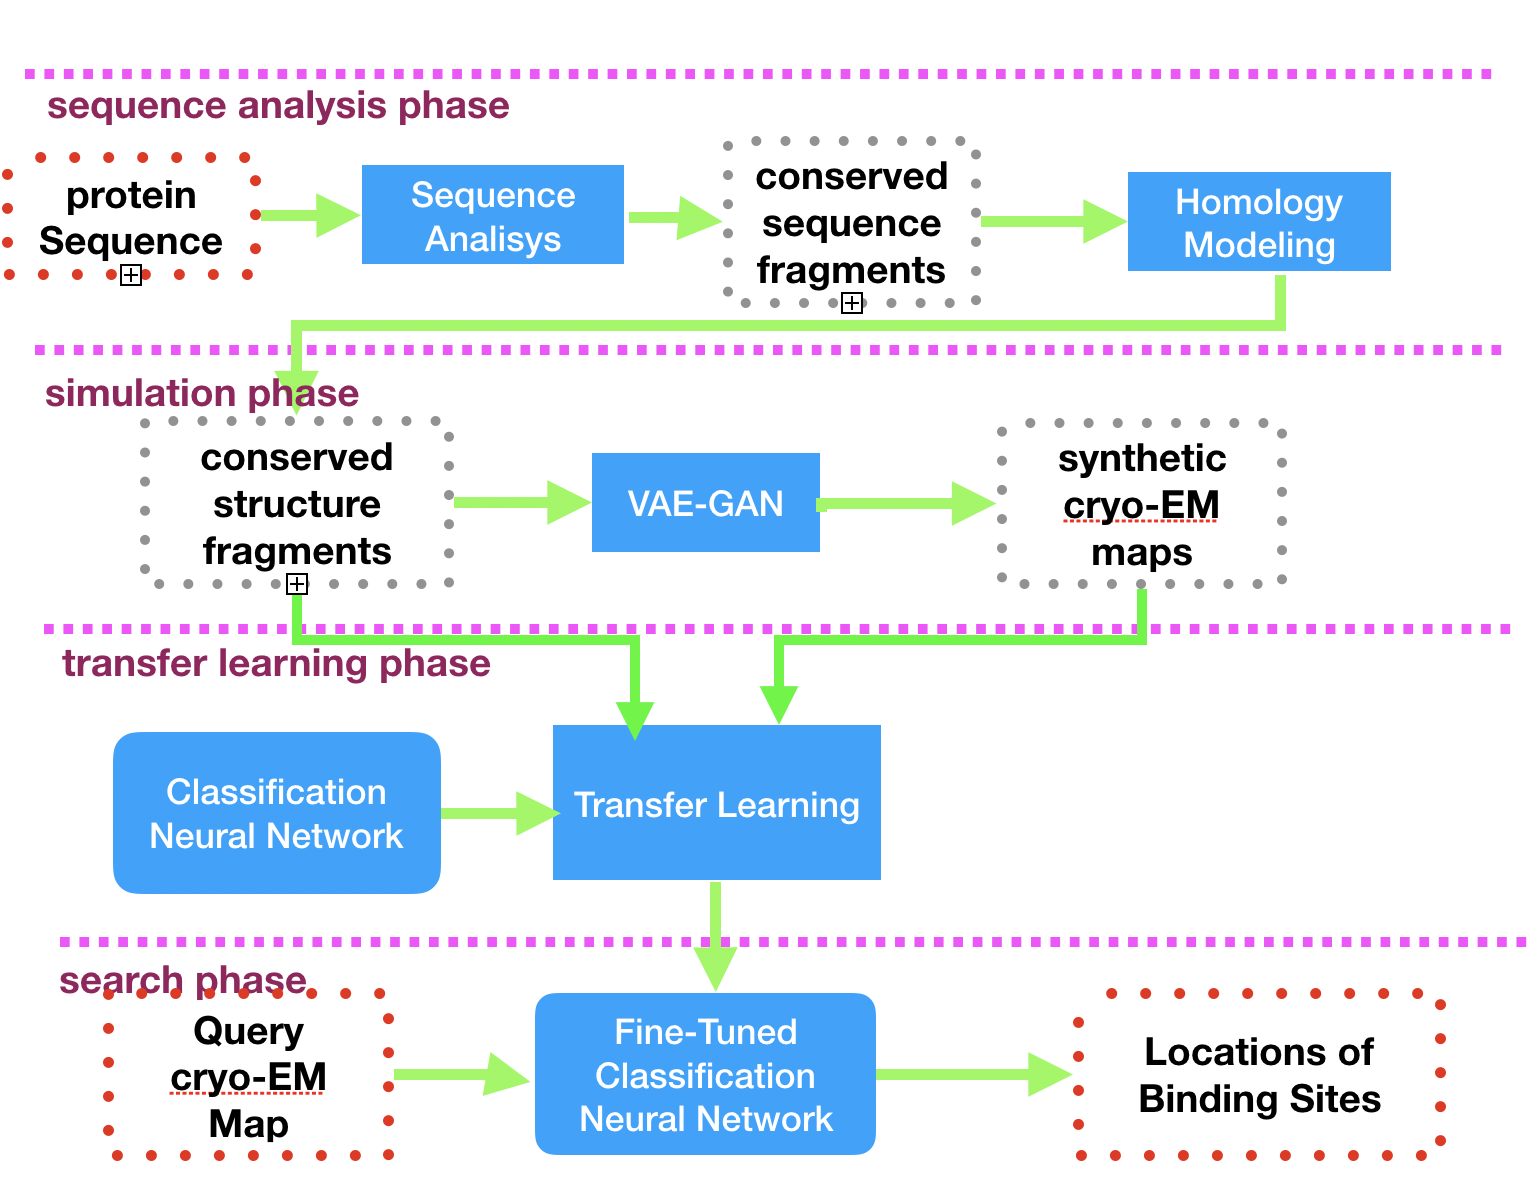
\includegraphics[scale=0.4]{picsnew/sch4.png}
  \caption{Finding Conserved Structures}\label{f:det_scheme4}
\end{figure}

\section{Summary}
As the time and cost of cryo electron microscopy experiments reduce , the ability of automatic structural analysis of experimental results becomes invaluable. 
We aim to show the potential of Deep Learning methods for analysis of cryo-EM maps.
We proposed a number of algorithms that using DL extract structural information from a cryo EM maps of high and intermediate resolution.
The proposed methods can be used for obtaining an atomic model of a molecule and for revealing its functionality.
In the final stage of our  work we will make an effort to integrate the proposed tools into an ab-initio modelling algorithm. 

\bibliography{references}{}
\bibliographystyle{plain}

\end{document}

